\documentclass[tikz, dvipsnames]{standalone}

\usepackage{amsmath}
\usepackage{amssymb}

\begin{document}
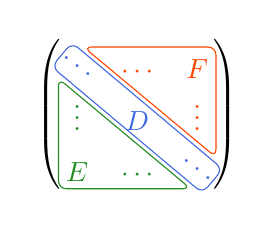
\begin{tikzpicture}
\node at (0,0.045) {$\begin{pmatrix}\textcolor{RoyalBlue}{\ddots} & \textcolor{OrangeRed}{\cdots} & \textcolor{OrangeRed}{F}\\ \textcolor{ForestGreen}{\vdots} & \textcolor{RoyalBlue}{D} & \textcolor{OrangeRed}{\vdots}\\\textcolor{ForestGreen}{E} &\textcolor{ForestGreen}{\cdots} & \textcolor{RoyalBlue}{\ddots}\end{pmatrix}$};
\draw[rotate=-40,rounded corners=1mm,RoyalBlue] (-1.25,-0.2) rectangle (1.25,0.2);
\draw[rounded corners=1mm,OrangeRed] (-0.68,0.9) -- (1,0.9) -- (1,-0.5) -- cycle;
\draw[rounded corners=1mm,ForestGreen] (0.68,-0.9) -- (-1,-0.9) -- (-1,0.5) -- cycle;
%\draw[very thin] (-2,0) -- (2,0) (0,-2) -- (0,2);
\end{tikzpicture}
\end{document}